\chapter{Non-switching-isomorphic graphs}

Considering one underlying graph, the number of signed graphs is simply too big for an efficient analysis. Filtering them for switching-isomorphism reduces them to manageable amounts and ensures clean and usable data. Bagheri, Moghaddamfar, Ramezani\cite{switching-isomorphic} establish a method of determining the non-switching-isomorphic signed graphs based on the action of its automorphism group. Our aim is to automate this process using a different idea and making analysis of small cubic signed graphs possible.

\section{Switching equivalence}

Two signed graphs are \textit{switching-equivalent} if one can be obtained from the other with a series Given an underlying graph $G$ there are $2^{|E_G|}$ possible signed graphs constructed from $G$. However, provided that $G$ is connected, only $2^{|E_G| - |V_G| + 1}$ or them are mutually non-switching equivalent.

\begin{theorem}\label{lem1:eq-classes}
    Let $G$ be a simple unsigned connected graph with $n$ vertices and $m$ edges. There are $2^{m - n + 1}$ mutually non-switching equivalent graphs on $G$.
\end{theorem}

\textit{Proof.} Bagheri, Moghaddamfar, Ramezani\cite{switching-isomorphic} prove this theorem but we present a simpler version. The idea is to use a spanning tree $S \subseteq G$ and show that each switching equivalence class of $G$ has exactly one element that is all-positive on $S$. Since $S$ contains $n - 1$ edges, there are $2^{m - (n - 1)}$ different graphs all-positive on $S$. Suppose we have a signed graph $\Gamma$ all-positive on $S$ and we switch some vertices. If we switch no vertices or all vertices, the graph stays the same, so we will have a non-empty set of switched vertices $A$ and a non-empty set of unswitched vertices $B$. At least one edge of $S$ must have one end in $A$ and the other end in $B$, otherwise $G$ would not be connected or $S$ would not be a spanning tree. After this switching all edges with both ends in either $A$ or $B$ will retain the same sign (not reversed or reversed twice) and edges with one end in $A$ and on end in $B$ will have its sign reversed. Therefore every possible switching from $\Gamma$ will result in a graph that is not all-positive on $S$. \qed

We use this approach to reduce the number of signed graphs that need to be filtered for isomorphisms.

\section{Isomorphism}

A \textit{canonical form} of a graph $G$ is a graph isomorphic to $G$ such that each other graph isomorphic to $G$ has the same canonical form. Since there are known ways of converting unsigned graphs to canonical forms\cite{nauty}, we aim to define a conversion from signed graphs to unsigned graphs such that two signed graphs are switching-isomorphic if and only if they are isomorphic after the conversion.

The \textit{cycle space} of a graph is the collection of its Eulerian (even-degree) spanning subgraphs. It can be described as a vector space over the two-element Galois field: the elements are Eulerian subgraphs, the additive operation is symmetric difference (given two graphs the result contains edges that are in exactly one of them) and trivial scalar multiplication. Cycles are trivial elements of the cycle space because each Eulerian subgraph is the sum of some cycles in the context of this vector space. Consequently, there must be a \textit{cycle basis}, a set of linearly independent cycles that generates this cycle space.

\section{Transformation}

Cycles behave well under both isomorphism and vertex switching. Two isomorphic graphs have the same number of cycles of the same length and the balance of cycles is consistent under vertex switching so two isomorphic \textit{signed} graphs will have the same number of balanced and unbalanced cycles of the same length. The idea is to consider all cycles of progressively bigger length until we construct a set that generates the whole cycle space. Given this set of cycles we construct an unsigned graph and show that two signed graphs are switching-isomorphic if and only if they are isomorphic after processed in the following way.

\begin{theorem}\label{lem2:conversion}
    Starting with the unsigned underlying graph, for each cycle we add one \textit{cycle vertex} and connect it to each vertex of the original cycle. We represent their balance with \textit{tails}, each balanced cycle vertex will have a tail of length one and unbalanced cycles will have a tail of length two. Signed graphs with minimal degree three or more are switching-isomorphic if and only if they are isomorphic after processed this way.
\end{theorem}

\textit{Proof.} The balance tails are either a vertex of degree one or an additional vertex of degree two. Since degrees of vertices are preserved under isomorphism and both original vertices vertices and cycle vertices have minimal degree three, balanced tails will be projected only onto balanced tails and unbalanced tails onto unbalanced tails. By extension cycle vertices will be projected only onto cycle vertices, because each tail is connected to exactly one cycle vertex. Consequently the original vertices will also be projected only onto each other.

Any isomorphism between two signed graphs transformed this way consists of two parts. Based on the above, reduction to the set of original vertices results in a correct isomorphism between the underlying graphs. The part that is projecting cycle vertices and tails ensures that the signatures are switching-equivalent. \qed

\begin{figure}[h]
    \centering
    \begin{tikzpicture}
        \begin{scope}[every node/.style={circle,draw,fill=black}]
            \node (1)  at (0,0) {};
            \node (2)  at (3,0) {};
            \node (3)  at (0,-3) {};
            \node (4)  at (3,-3) {};
        \end{scope}
        \node (cheat) at (-1.5,1.2) {};
        \node (cheat2) at (3.8,-5.2) {};
        \begin{scope}[every edge/.style={draw,very thick}]
            \path
                (1) edge (2)
                (2) edge [dashed] (3)
                (3) edge (1)
                (2) edge (4)
                (3) edge [dashed] (4);
        \end{scope}
    \end{tikzpicture}
    \hspace{0.1\textwidth}
    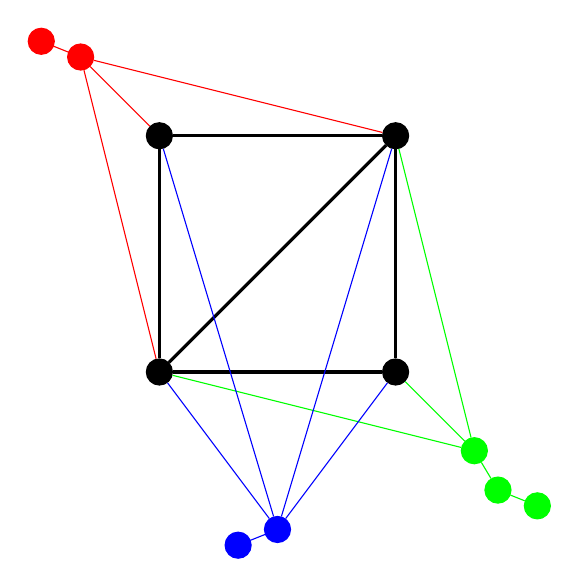
\begin{tikzpicture}
        \begin{scope}[every node/.style={circle,draw,fill=black}]
            \node (1)  at (0,0) {};
            \node (2)  at (3,0) {};
            \node (3)  at (0,-3) {};
            \node (4)  at (3,-3) {};
        \end{scope}
        \begin{scope}[every node/.style={circle,draw}]
            \node (11) [fill=red,color=red]  at (-1,1) {};
            \node (12) [fill=green,color=green] at (4,-4) {};
            \node (13) [fill=blue,color=blue] at (1.5,-5) {};
            \node (14) [fill=green,color=green] at (4.3,-4.5) {};
            \node (15) [fill=green,color=green] at (4.8,-4.7) {};
            \node (16) [fill=red,color=red] at (-1.5,1.2) {};
            \node (17) [fill=blue,color=blue] at (1,-5.2) {};
        \end{scope}
        \begin{scope}[every edge/.style={draw,very thick}]
            \path
                (1) edge (2)
                (2) edge (3)
                (3) edge (1)
                (2) edge (4)
                (3) edge (4);
        \end{scope}
        \begin{scope}[every edge/.style={draw,thin,color=red}]
            \path
                (1) edge (11)
                (2) edge (11)
                (3) edge (11)
                (11) edge (16);
        \end{scope}
        \begin{scope}[every edge/.style={draw,thin,color=green}]
            \path
                (2) edge (12)
                (3) edge (12)
                (4) edge (12)
                (12) edge (14)
                (14) edge (15);
        \end{scope}
        \begin{scope}[every edge/.style={draw,thin,color=blue}]
            \path
                (1) edge (13)
                (2) edge (13)
                (3) edge (13)
                (4) edge (13)
                (13) edge (17);
        \end{scope}
    \end{tikzpicture}
    \caption[Example of transformation]{Example of a transformation to an unsigned graph.}
\end{figure}
